\PassOptionsToPackage{table}{xcolor}

\documentclass[10pt]{beamer}

%\usepackage{lmodern}
%\usepackage[labelformat=empty,font=scriptsize,skip=0pt,justification=justified,singlelinecheck=false]{caption}

%\usepackage{paralist}
%\usepackage{amsmath}% http://ctan.org/pkg/amsmath
%\usepackage{amsfonts}% http://ctan.org/pkg/amsfonts

%\usepackage[font=scriptsize]{caption}

%\usepackage{hyperref}
\usepackage{amssymb,amsmath,amsfonts,eurosym,geometry,graphicx,caption,color,setspace,
comment,footmisc,caption,pdflscape,array}
\usepackage{booktabs}   % for nice tables
\usepackage{multirow}
%\usepackage[round]{natbib}
\setbeamertemplate{caption}[numbered]
\usepackage[export]{adjustbox}

\usepackage[skip=1pt]{caption}
%\usepackage[capposition=top]{floatrow}

%\usepackage[caption = false]{subfig}
%\usepackage{floatrow}
\usepackage[capposition=bottom]{floatrow}

\usepackage{graphicx}
\usepackage{tabularx}
%\usepackage{threeparttable}
\usepackage{float}
\usepackage{mwe}
%\usepackage{subfig}
%\usepackage{polyglossia}
\usepackage{subcaption}
\setlength{\abovecaptionskip}{2pt}
%\usepackage[tight,TABTOPCAP]{subfigure}
\usepackage[round]{natbib}

\usepackage{multicol, latexsym, amsmath, amssymb}

\usepackage[normalem]{ulem}
\useunder{\uline}{\ul}{}
\usepackage{booktabs,caption}
\usepackage[flushleft]{threeparttable}

\usepackage{graphics}

\usepackage{longtable}

\usepackage{float}

\usepackage{amsbsy} %boldsymbol

%%in case of outdated TEX Live
\usepackage{lmodern}

\usepackage{appendixnumberbeamer}

%\graphicspath{{figures/}{../figures/}{D:/Presentations\figures/}}
\usepackage[normalem]{ulem}

\usepackage{siunitx}
\sisetup{
	round-mode          = places, % Rounds numbers
	round-precision     = 4, % to 2 places
}

\mode<presentation> {

% The Beamer class comes with a number of default slide themes
% which change the colors and layouts of slides. Below this is a list
% of all the themes, uncomment each in turn to see what they look like.

%\usetheme{default}
%\usetheme{AnnArbor}
%\usetheme{Antibes}
%\usetheme{Bergen}
%\usetheme{Berkeley}
%\usetheme{Berlin}
%\usetheme{Boadilla}
%\usetheme{CambridgeUS}
%\usetheme{Copenhagen}
%\usetheme{Darmstadt}
%\usetheme{Dresden}
%\usetheme{Frankfurt}
%\usetheme{Goettingen}
%\usetheme{Hannover}
%\usetheme{Ilmenau}
%\usetheme{JuanLesPins}
%\usetheme{Luebeck}
\usetheme{Madrid}
%\usetheme{Malmoe}
%\usetheme{Marburg}
%\usetheme{Montpellier}
%\usetheme{PaloAlto}
%\usetheme{Pittsburgh}
%\usetheme{Rochester}
%\usetheme{Singapore}
%\usetheme{Szeged}
%\usetheme{Warsaw}

% As well as themes, the Beamer class has a number of color themes
% for any slide theme. Uncomment each of these in turn to see how it
% changes the colors of your current slide theme.

%\usecolortheme{albatross}
%\usecolortheme{beaver}
%\usecolortheme{beetle}
%\usecolortheme{crane}
%\usecolortheme{dolphin}
%\usecolortheme{dove}
%\usecolortheme{fly}
%\usecolortheme{lily}
%\usecolortheme{orchid}
%\usecolortheme{rose}
%\usecolortheme{seagull}
%\usecolortheme{seahorse}
%\usecolortheme{whale}
%\usecolortheme{wolverine}

%\setbeamertemplate{footline} % To remove the footer line in all slides uncomment this line
%\setbeamertemplate{footline}[page number] % To replace the footer line in all slides with a simple slide count uncomment this line

%\setbeamertemplate{navigation symbols}{} % To remove the navigation symbols from the bottom of all slides uncomment this line
}
\usecolortheme{seahorse}

\usepackage{graphicx} % Allows including images
\usepackage{booktabs} % Allows the use of \toprule, \midrule and \bottomrule in tables

\usepackage{arydshln} %can use hdashline

\setbeamertemplate{footnote}{%
  \hangpara{2em}{1}%
  \makebox[2em][l]{\insertfootnotemark}\footnotesize\insertfootnotetext\par%
}
%----------------------------------------------------------------------------------------
%	TITLE PAGE
%----------------------------------------------------------------------------------------

\title[Credit \& Housing]{Housing and Credit Cycles} % The short title appears at the bottom of every slide, the full title is only on the title page

\author{Nam Nguyen} % Your name
\institute[nguyent3@uwm.edu]
 % Your institution as it will appear on the bottom of every slide, may be shorthand to save space
{
	
	
	\medskip 
	
	Department of Economics \\  
	University of Wisconsin - Milwaukee \\ % Your institution for the title page
%	\textit{estorm@carleton.edu} % Your email address
	
	\bigskip
	
	 Paper Presentation for: \\
		\smallskip
	\textit{Weekly Friday Meeting}
}


\date{February 05, 2021} % Date, can be changed to a custom date

\begin{document}

\begin{frame}
\titlepage % Print the title page as the first slide
\end{frame}



%----------------------------------------------------------------------------------------
%	PRESENTATION SLIDES
%----------------------------------------------------------------------------------------

%------------------------------------------------

%\begin{frame} 
%\frametitle{Overview}

%\textbf{Core theme in a nutshell}
%\bigskip
%\begin{itemize}
%\item [$\Rightarrow$] Refined measurement of Skills using detailed Task information and how they translate into Wage differences
%\end{itemize}
 
%\bigskip
 
%\begin{enumerate}
%\item Comparison of individual (self-reported) vs commonly used occupation-level task data (derived from external assessments of labor market experts)
%\item Implications of variation in individual tasks on the Native-Foreign Wage Gap with an emphasis on distributional effects
%\end{enumerate} 
 
%\bigskip
 
%\begin{itemize}
%\item Primary data set
%	\begin{itemize}
%	\item German employment surveys, assembled by the Federal Institute for Vocational Education (BIBB), the Institute of Employment Research (IAB) and the Federal Institute of Occupational Safety and Health (BAuA)
%	\item Provide self-reported information about job-related activities at the individual level
%	\end{itemize}
%\end{itemize}
 
 
%\end{frame}

%------------------------------------------------
%------------------------------------------------



%\begin{frame} 
%	\frametitle{Motivation}
%	
%
%%	\begin{figure}[H]
%%		\centering
%%		\begin{minipage}{0.90\textwidth} % choose width suitably
%%			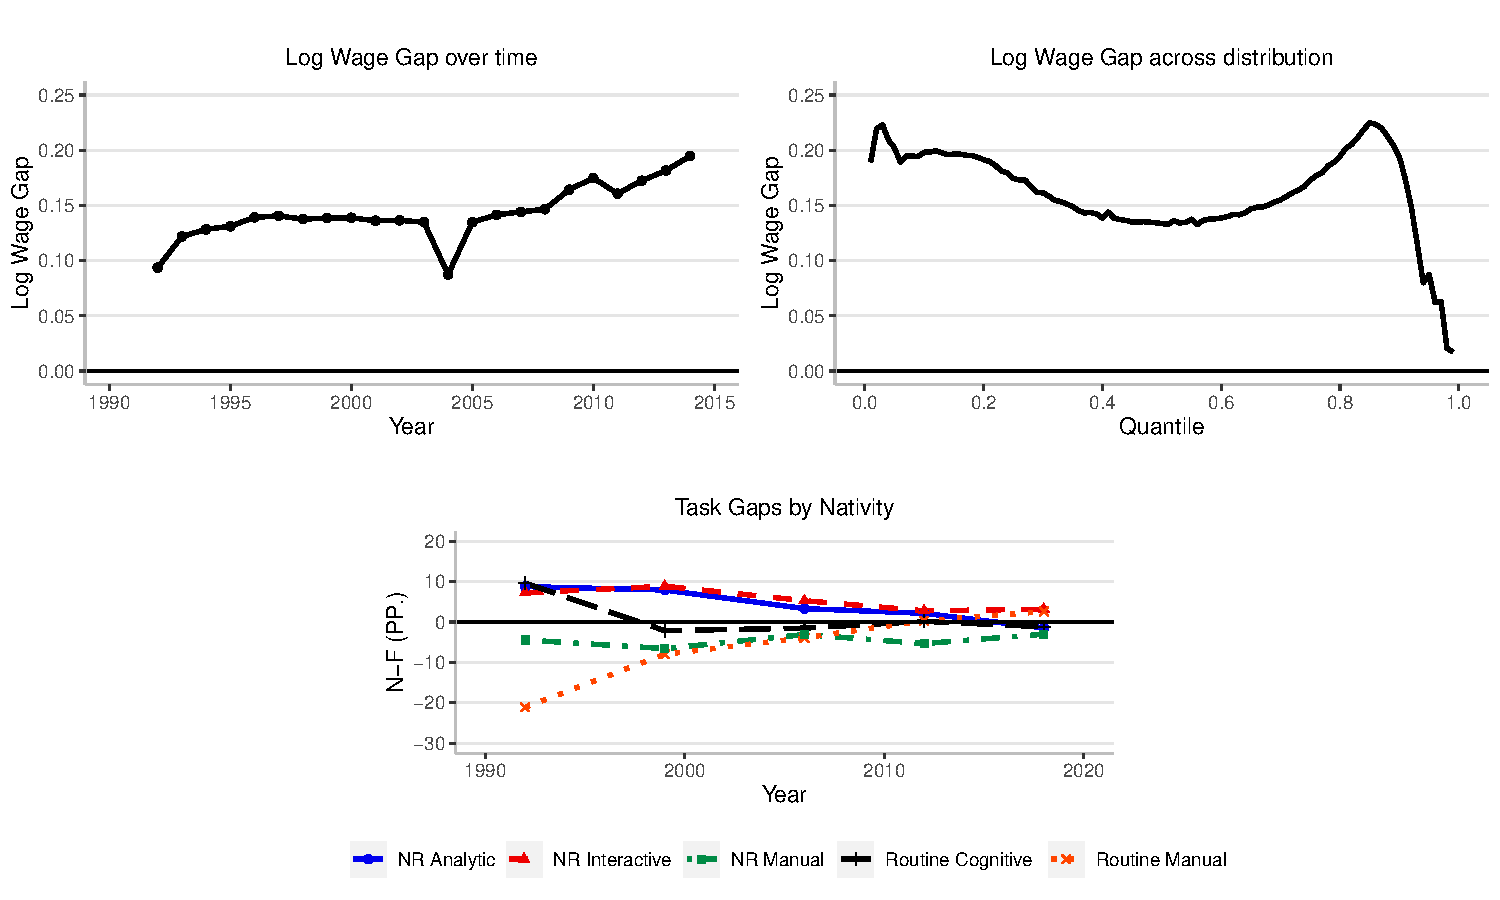
\includegraphics[width=0.90\linewidth]{wgap_tgap}
%%			\caption{  Native-Foreign (NF) Wage \& Task Gap in Germany, 1992-2018 \\ 
%%				\medskip \centering \tiny Source: SIAB-R 7514, BIBB/IAB/BAuA \label{fig:wage_gap}}
%%			{\footnotesize \tiny NOTE. \textemdash ``NR'' stands for Non-Routine Activities. NR Analytic and NR Interactive can be subsumed under \textit{Abstract} tasks, involving lots of problem-solving skills. Routine Cognitive and Routine Manual can be subsumed under \textit{Routine} tasks, characterized by various repetitive steps. NR \textit{Manual} involves activities requiring hand-eye coordination, which are difficult to automate.  \par}
%%			%{\caption  {Contributions of Task Variation Within Occupations to the explained Native-Foreign Wage Gap with base task group Routine Manual, 1992-2018 \label{fig:wgap_within_baserm}}}
%%		\end{minipage}
%%	\end{figure}
%	
%
%\end{frame}

%------------------------------------------------
\begin{frame} 
	\frametitle{Motivation}
	
	
	\begin{itemize}
		\item 	The study of housing prices has become more important in understanding financial market stability. We also observed increasing use of monetary policies.
	\end{itemize}
	
\end{frame}

%------------------------------------------------
\begin{frame}
	\frametitle{Contributions}
	
	\begin{enumerate}
		\item \textbf{Relationship between housing prices and household credit}
		\begin{itemize}
			\item Apply Unobserved Component Model (Morley 2007) to extract information about trends and cycles.
			\medskip
			\item[$\Rightarrow$] Focus on the dynamics between transitory cycle components.
		\end{itemize} 
		
		\smallskip
		
		\item \textbf{Specify cycles to be VAR process (cross-cycle) rather than univariate AR process}
		\begin{itemize}
			\medskip
			\item[$\Rightarrow$] Test if past movement of one cycle has predictive power over another cycle.
%			\item[$\Rightarrow$] Conventional decomposition methods such as Oaxaca-Blinder (OB) understate the impact of tasks on wage gaps
		\end{itemize} 
%		
%		\smallskip
%		
%		\item \textbf{Between-Occupation vs Within-Occupation Contributions}
%		\begin{itemize}
%			\item Occupational segregation: $\geq 70\%$ 
%			\item \underline{Within-Occupation specialization}: $\geq 10\%$   %only for high-wage earners
%			\medskip
%			\item[$\Rightarrow$] Focus on occupational segregation alone understates degree of task specialization between N \& F (e.g., \textit{Peri \& Sparber 2009, 2011})
%		\end{itemize} 
%				
		
	\end{enumerate}	
	
\end{frame}

%------------------------------------------------
\begin{frame} 
	\frametitle{Data}
	
	\begin{itemize}	
		\item Bank of International Settlement (BIS)
		\begin{itemize}
			\item[-] Household Credit to GDP: Total Credit to non-financial sector (household)
			\item[-] House Price Index: Residential property prices: selected series (real value)
		\end{itemize}
	
		\item 2 countries: US \& GB
		\item Time frame: 1990:Q1 - 2019:Q3 
		
	\end{itemize}
	
	
%	\begin{figure}[H]
%		\begin{adjustbox}{addcode={\begin{minipage}{\width}}{\caption{From Activities to Tasks: Construction of the Task Content \label{fig:tasks_creation}
%				}\end{minipage}},center}
%			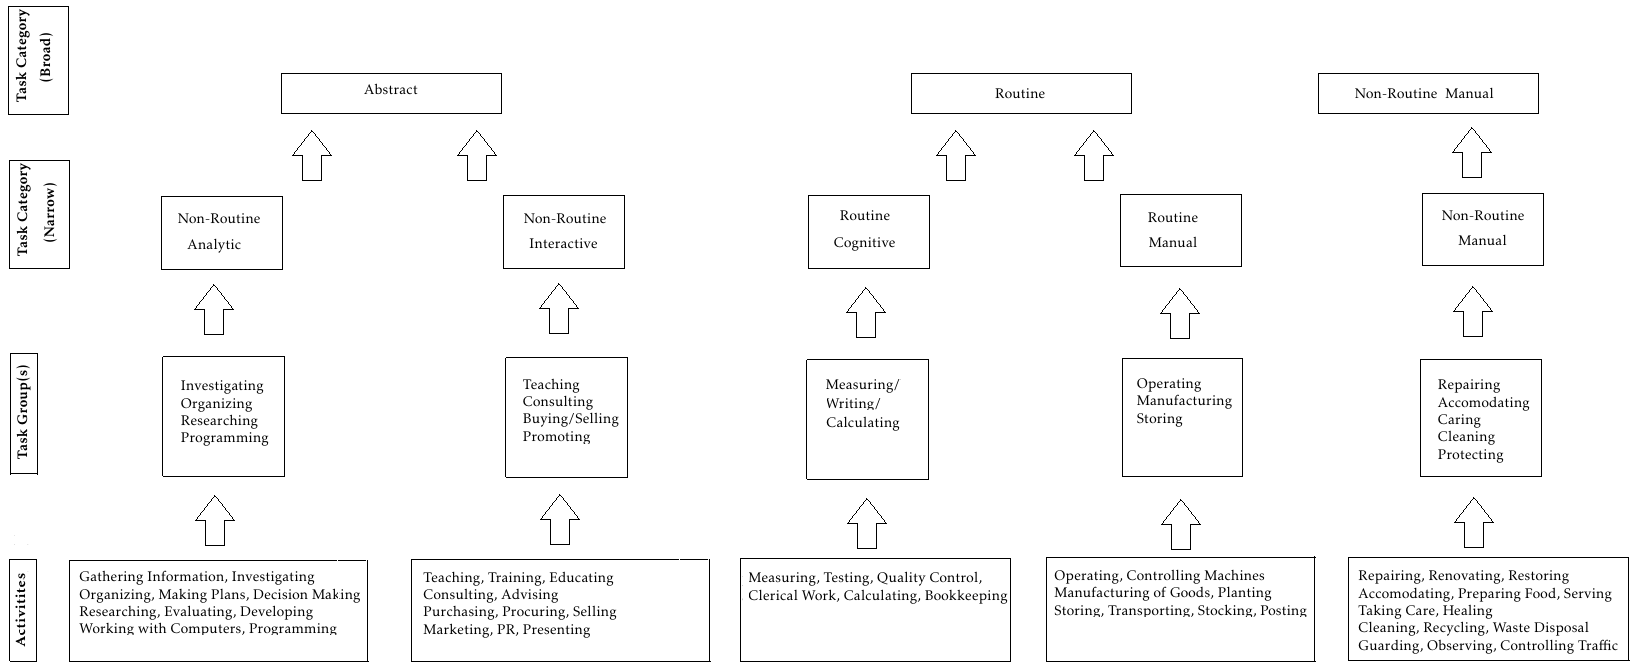
\includegraphics[scale=.36]{task_aggregation_illustration_FINAL}%
%		\end{adjustbox}
%	\end{figure}
	
	%,rotate=90
	
\end{frame}

%------------------------------------------------
\begin{frame} 
	\frametitle{Methodology}
	
	\textbf{Main Model: Unobserved Component Model}
	

\begin{align}
	100*ln \frac{Credit}{GDP} &= y_t = \tau_{yt} + c_{yt}
	\\
	100*ln HPI &= h_t = \tau_{ht} + c_{ht}
\end{align}

	\begin{itemize}
	\item\textbf{\textit{Trends:}}
	\end{itemize}
	\begin{align}
		\tau_{yt} &= \tau_{yt-1} + \eta_{yt}, &\eta_{yt} \sim iidN(0,\sigma^2_{\eta y})
		\\
		\tau_{ht} &= \tau_{ht-1} + \eta_{ht}, &\eta_{ht} \sim iidN(0,\sigma^2_{\eta h})	
	\end{align}
	
\end{frame}

%------------------------------------------------
\begin{frame} 
	\frametitle{Methodology: UC Model}
		
	\begin{itemize}
		\item\textbf{\textit{Cycles:}}
	\end{itemize}

	\begin{align}
		c_{yt} &= \phi^1_{y}c_{yt-1}  
		+ \phi^2_{y}c_{yt-2}  
		+ \phi^{x1}_{y}c_{ht-1} 
		+ \phi^{x2}_{y}c_{ht-1} 
		+ \varepsilon_{yt},
		&\varepsilon_{yt} \sim iidN(0,\sigma^2_{\varepsilon y})		   
		\\
		c_{ht} &= \phi^1_{h}c_{ht-1}  
		+ \phi^2_{h}c_{ht-2}
		+ \phi^{x1}_{h}c_{yt-1}  
		+ \phi^{x2}_{h}c_{yt-1}  
		+ \varepsilon_{ht},
		&\varepsilon_{ht} \sim iidN(0,\sigma^2_{\varepsilon h})
	\end{align}
	
\end{frame}

%------------------------------------------------

\begin{frame}[label=StateSpace]  
	\frametitle{Methodology: UC Model}
	
	\textbf{State Space Representation}
	
	\textit{Transition equation:}
	\begin{align}
		\beta_t = F\beta_{t-1} + \tilde{v}_t
	\end{align}
	
	Where the transitory components are:
	
	\begin{align}
		\begin{bmatrix}
			\tau_{yt}	\\
			c_{yt}		\\
			c_{yt-1}		\\
			\tau_{ht}	\\
			c_{ht}		\\
			c_{ht-1}		
		\end{bmatrix}
		=
		%F matrix
		\begin{bmatrix}
			1	& 0	& 0	& 0	& 0	& 0	\\
			0	& \phi^1_y	& \phi^2_y	& 0	& \phi^{x1}_y	& \phi^{x2}_y	\\
			0	& 1	& 0	& 0 & 0 & 0  \\
			0	& 0	& 0	& 1	& 0	& 0 \\
			0	& \phi^{x1}_h	& \phi^{x2}_h	& 0 &\phi^1_h	& \phi^2_h	\\
			0	& 0	& 0	& 0 & 1 & 0
		\end{bmatrix}
		%Bt-1 matrix
		\begin{bmatrix}
			\tau_{yt-1}	\\
			c_{yt-1}		\\
			c_{yt-2}		\\
			\tau_{ht-1}	\\
			c_{ht-1}		\\
			c_{ht-2}		
		\end{bmatrix}
		+
		\begin{bmatrix}
			\eta_{yt}	\\
			\varepsilon_{yt}		\\
			0	\\
			\eta_{ht}	\\
			\varepsilon_{ht}		\\
			0	
		\end{bmatrix}
	\end{align}
	
\hyperlink{Reg_US}{\beamergotobutton{Regression results}} 	
	
\end{frame}


%------------------------------------------------



\begin{frame}[label=CovarMatrix]  
	\frametitle{Methodology UC Model}
	
	
		\textit{The covariance matrix for $\tilde{v}_t$, denoted Q, is: }
\begin{align}
	Q = 
	\begin{bmatrix}
		\sigma^2_{\eta y}	& 0	 &0 & \sigma_{\eta y \eta h}	& 0	& 0	\\
		0	& \sigma^2_{\varepsilon y}	& 0	& 0	& \sigma_{\varepsilon y \varepsilon h}	& 0	\\
		0	&	0	& 0 & 0 & 0 & 0	\\
		\sigma_{\eta y \eta h}	& 0	& 0	& \sigma^2_{\eta h}	& 0	& 0	\\
		0	& \sigma_{\varepsilon y \varepsilon h}	& 0	& 0	& \sigma^2_{\varepsilon h}		& 0	\\
		0	&0	& 0	& 0
		& 0	& 0
	\end{bmatrix}
\end{align}
	

\hyperlink{Reg_US}{\beamergotobutton{Regression results}} 	
	
\end{frame}

%------------------------------------------------
\begin{frame}
	\frametitle{Methodology: UC Model}
			\textit{Constraint estimation}
			\begin{itemize}
				\item Conventional VAR models constrain parameters using a transformation function so that they lie in feasible region.
				\item[-] I ran into problems of setting up a working prior.
			\end{itemize}
		
			\begin{itemize}
			\item \textbf{What I do:} Add a penalty term on magnitude of cycles in the log-likelihood function:
			 \begin{align*}
				l(\theta) = -\frac{1}{2}\sum_{t=1}^{T}ln\lbrack(2\pi)^2|f_{t|t-1}|\rbrack
				-\frac{1}{2}\sum_{t=1}^{T}\eta'_{t|t-1}f^{-1}_{t|t-1}\eta_{t|t-1}
				\\ - 0.003*\sum_{t=1}^{T}(c_{yt}^2+c_{ht}^2)
			\end{align*}
		\end{itemize}
	
%	\begin{figure}[H]
%		\begin{minipage}{0.95\textwidth} % choose width suitably
%			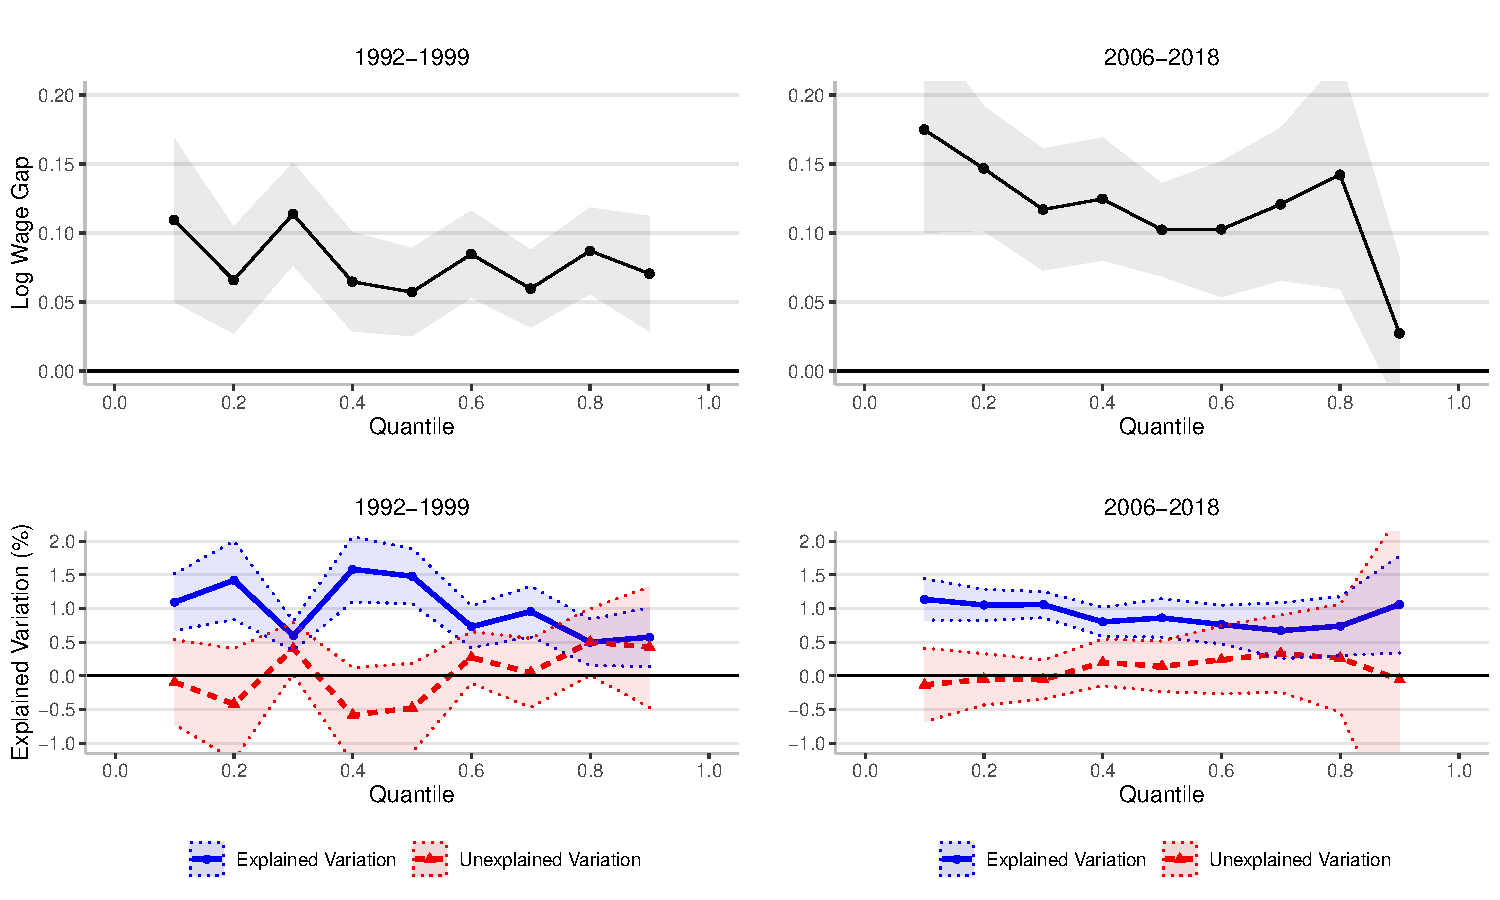
\includegraphics[scale=0.4]{nfgap_t} \\
%			{\footnotesize \tiny NOTE. \textemdash Point estimates are displayed with a 95\% Confidence Interval. \par}
%			\caption{\centering German Native-Foreign Wage Gap by sub-samples, 1992-2018 \label{fig:wgap_subs}}
%		\end{minipage}
%	\end{figure}
	
	
	
\end{frame}

%------------------------------------------------
\begin{frame}
	\frametitle{Methodology: UC Model}
	\textit{Stationary Region AR(2) series}
	\begin{itemize}
		\item[-] Visualize using isStable() function in Matlab
	\end{itemize}

	
	\begin{figure}[H]
		\begin{minipage}{0.95\textwidth} % choose width suitably
			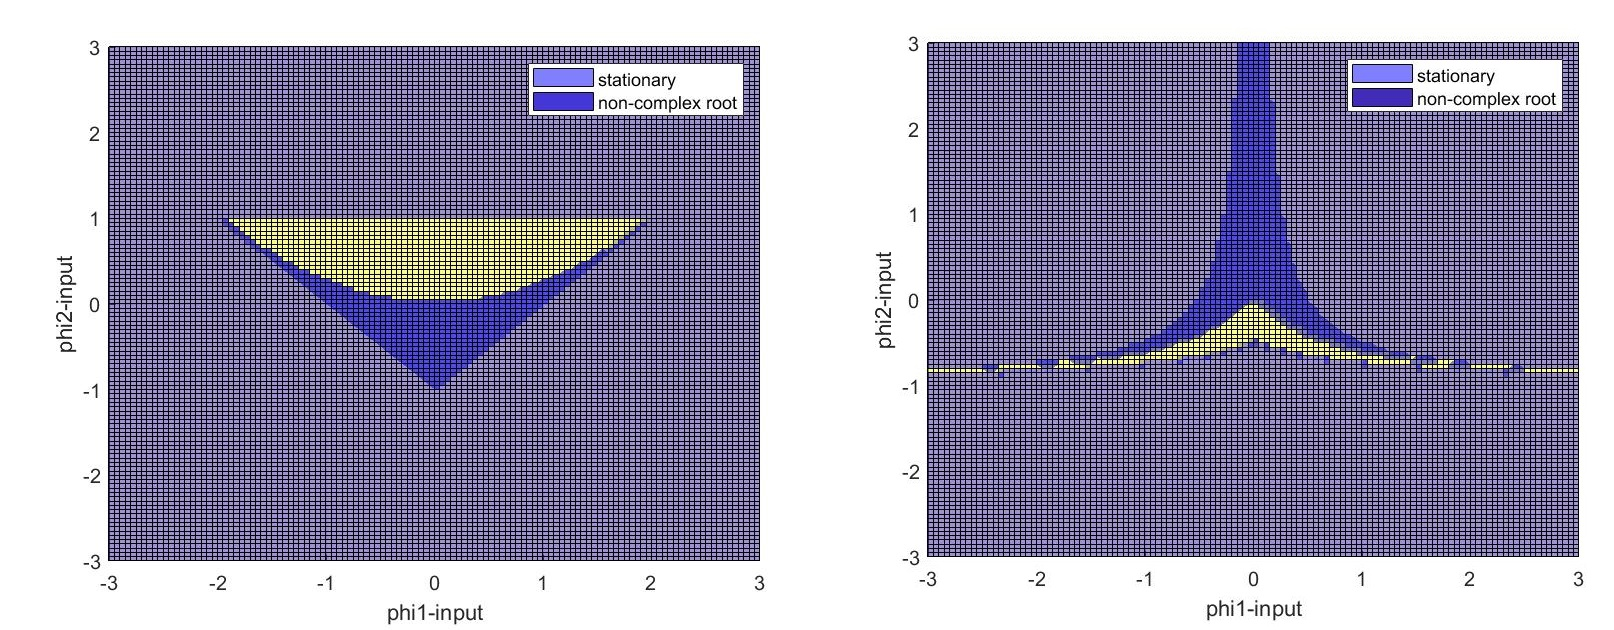
\includegraphics[scale=0.5]{stationary1.jpg}
		\end{minipage}
	\end{figure}
		
\end{frame}
 
%------------------------------------------------

\begin{frame}[label=Reg_US]
	\frametitle{Key Results Regression Table: United States}


\resizebox{\linewidth}{!}{
				\rowcolors{2}{gray!10}{white}
	\begin{tabular}{@{}lSSSSSS@{}}
		\toprule
		\multirow{1}{*}{Parameters} & \multicolumn{2}{c}{VAR(2)} & \multicolumn{2}{c}{VAR(2) 1st-cross-lag} & \multicolumn{2}{c}{VAR(2) 2-cross-lags} \\
		& \multicolumn{1}{l}{Estimate}     & \multicolumn{1}{l}{Std. Error}  & \multicolumn{1}{l}{Estimate}            & \multicolumn{1}{l}{Std. Error}         & \multicolumn{1}{c}{Estimate}            & \multicolumn{1}{c}{Std. Error}        \\ \midrule
		$\phi^1_{y}$                & 1.521670374  & 0.323602024 & 1.890301193         & 0.036315042        & 1.886592178         & 0.00028419        \\
		$\phi^2_{y}$                & -0.592177551 & 0.282758652 & -0.773199508        & 0.021652307        & -0.8941981          & 0.003233388       \\
		$\phi^{x1}_{y}$             &              &             & -0.012689515        & 0.001245419        & 0.04280046          & 0.000520376       \\
		$\phi^{x2}_{y}$             &              &             &                     &                    & -0.040322766        & 0.000876719       \\
		$\phi^1_{h}$                & 1.803961772  & 0.039406338 & 1.465513594         & 0.064627659        & 1.864726867         & 0.038659834       \\
		$\phi^2_{h}$                & -0.820986013 & 0.039263457 & -0.736886204        & 0.047825955        & -0.898033258        & 0.039051475       \\
		$\phi^{x1}_{h}$             &              &             & 2.576890191         & 1.642027848        & 0.089729346         & 0.11453162        \\
		$\phi^{x2}_{h}$             &              &             &                     &                    & -0.031982418        & 0.113620129       \\
		$\sigma_{ny}$               & 0.968115538  & 0.064573932 & 0.975833563         & 0.066722551        & 0.858997834         & 0.055437867       \\
		$\sigma_{ey}$               & 0.136584746  & 0.073940054 & 0.000413197         & 0.008728546        & 0.030583756         & 0.016664357       \\
		$\sigma_{nh}$               & 0.964325946  & 0.107167236 & 1.271977495         & 0.127987617        & 1.135553581         & 0.106041662       \\
		$\sigma_{eh}$               & 0.471089742  & 0.079046967 & 0.296047479         & 0.161613716        & 0.363776038         & 0.077466523       \\
		$\sigma_{eyeh}$             & -0.999391959 & 0.03023235  & -0.881232755        & 0.311836698        & -1                  & 5.19E-07          \\
		$\sigma_{nynh}$             & 0.464225409  & 0.094391207 &                     &                    &                     &                   \\
		Log-likelihood value        & -369.9163016 &             & -384.7973521        &                    & -363.3991125        &                   \\ \bottomrule
\end{tabular}}

	\hyperlink{StateSpace}{\beamergotobutton{StateSpace}}		

\end{frame}

%------------------------------------------------

\begin{frame}[label=Reg_GB]
	\frametitle{Key Results Regression Table: Great Britain}
	
	
	\resizebox{\linewidth}{!}{
				\rowcolors{2}{gray!10}{white}
		\begin{tabular}{@{}lSSSSSS@{}}
			\toprule
			\multirow{1}{*}{Parameters} & \multicolumn{2}{c}{VAR(2)} & \multicolumn{2}{c}{VAR(2) 1st-cross-lag} & \multicolumn{2}{c}{VAR(2) 2-cross-lags} \\
			& \multicolumn{1}{l}{Estimate}     & \multicolumn{1}{l}{Std. Error}  & \multicolumn{1}{l}{Estimate}            & \multicolumn{1}{l}{Std. Error}         & \multicolumn{1}{c}{Estimate}            & \multicolumn{1}{c}{Std. Error}        \\ \midrule
					$\phi^1_{y}$         & 1.254192973  & 0.190985842 & 1.25723532   & 0.060817683 & 1.150590314  & 0.176355128 \\
					$\phi^2_{y}$         & -0.26306956  & 0.205161023 & -0.169780952 & 0.09490575  & -0.29219579  & 0.186002808 \\
					$\phi^{x1}_{y}$      &              &             & -0.032263112 & 0.011998484 & -9.25E-05    & 0.040559508 \\
					$\phi^{x2}_{y}$      &              &             &              &             & 0.001258809  & 0.049929897 \\
					$\phi^1_{h}$         & 1.624898849  & 0.106882442 & 0.680349073  & 0.111110636 & 0.37903173   & 0.134445053 \\
					$\phi^2_{h}$         & -0.735672409 & 0.11638218  & -0.058077279 & 0.119413569 & -0.513222468 & 0.172990361 \\
					$\phi^{x1}_{h}$      &              &             & 1.095293496  & 0.644515947 & 1.042175029  & 0.959665092 \\
					$\phi^{x2}_{h}$      &              &             &              &             & -0.24951917  & 1.444350906 \\
					$\sigma_{ny}$        & 0.860787938  & 0.082136594 & 1.144314466  & 0.116163949 & 0.739935351  & 0.04023517  \\
					$\sigma_{ey}$        & 0.289375924  & 0.120450619 & 0.192749525  & 0.076274126 & 0.475181328  & 0.106178287 \\
					$\sigma_{nh}$        & 2.340082466  & 0.172292974 & 2.162565122  & 0.187483055 & 1.423757795  & 0.059105068 \\
					$\sigma_{eh}$        & 0.75058414   & 0.220465076 & 1.898423971  & 0.342466946 & 2.079589016  & 0.470123296 \\
					$\sigma_{eyeh}$      & 0.957116136  & 0.252780005 & 0.502139385  & 0.163311142 & 0.48533368   & 0.153929437 \\
					$\sigma_{nynh}$      & 0.591929269  & 0.07200974  &              &             &              &             \\
					Log-likelihood value & -410.01474   &             & -448.3113461 &             & -512.4696846 &                             \\ \bottomrule
	\end{tabular}}
	
	\hyperlink{StateSpace}{\beamergotobutton{StateSpace}}		

\end{frame}

%------------------------------------------------


%\begin{frame}
%	\frametitle{Key Results RIF Decomposition: Long-term Trends (Abstract Tasks)}


%\begin{figure}[H]
%			\begin{minipage}{0.95\textwidth} % choose width suitably
%				\centering
%	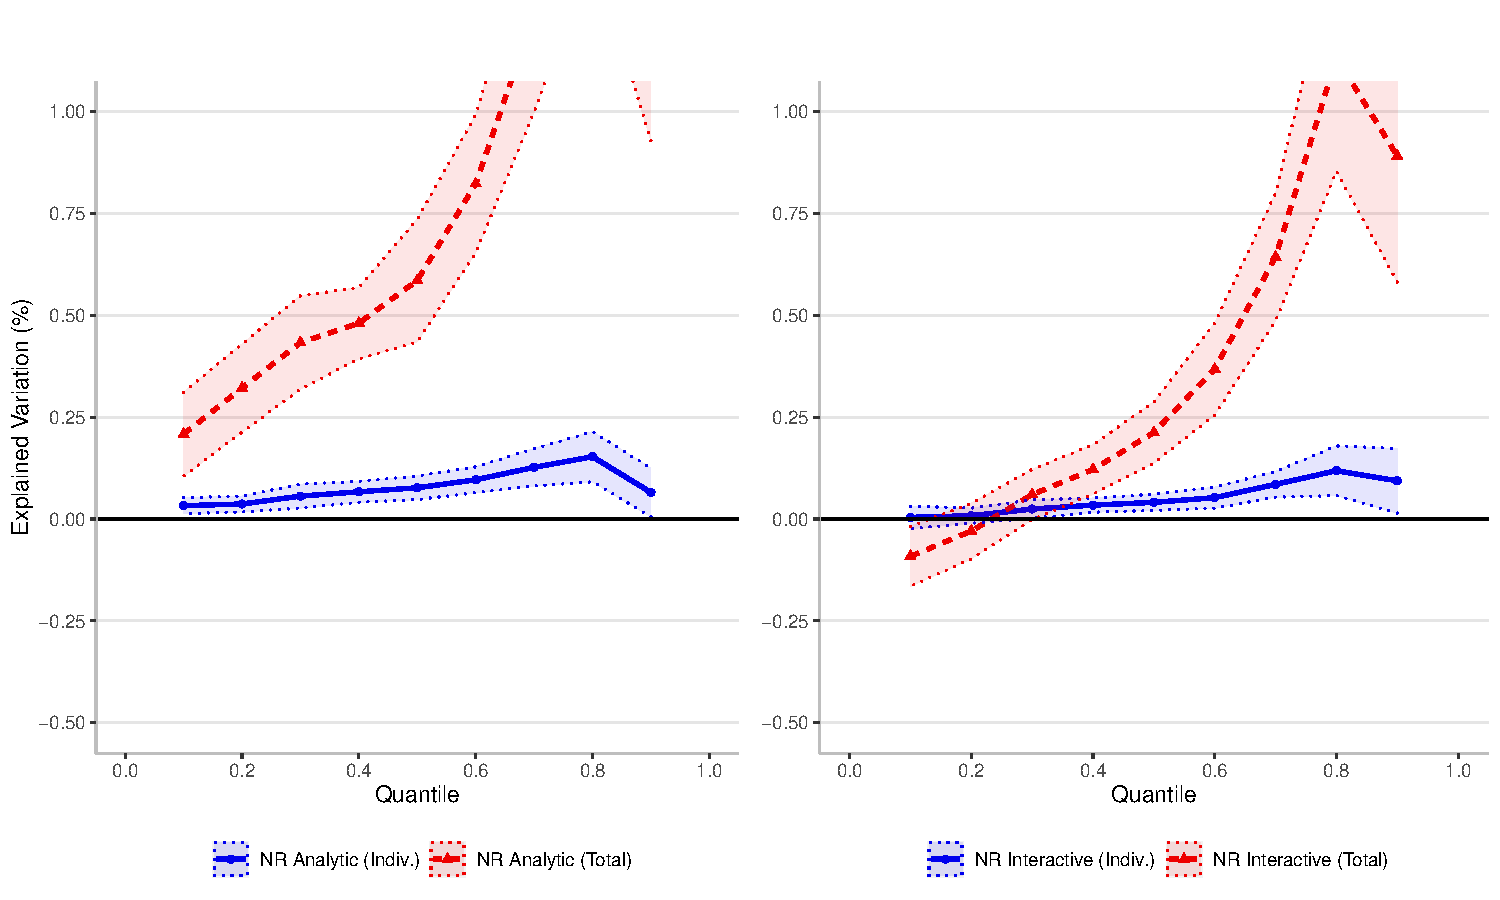
\includegraphics[scale=0.38]{rif_base_all_cog} \\
%	{\footnotesize \tiny NOTE. \textemdash The decomposition results are top-censored for clarity, i.e. cut off at contributions of 100\% to the explained wage gap.\par}
%	\caption{\centering Contributions of Individual-level variation in Abstract Tasks to the explained Native-Foreign Wage Gap, 1992-2018 \label{fig:wgap_indiv_occ}}
%		\end{minipage}
%\end{figure}


%\end{frame}

%------------------------------------------------


\begin{frame}
	\frametitle{Key Results Regression Graphs: United States}
	
	\begin{figure}[H]
		\begin{minipage}{0.95\textwidth} % choose width suitably
			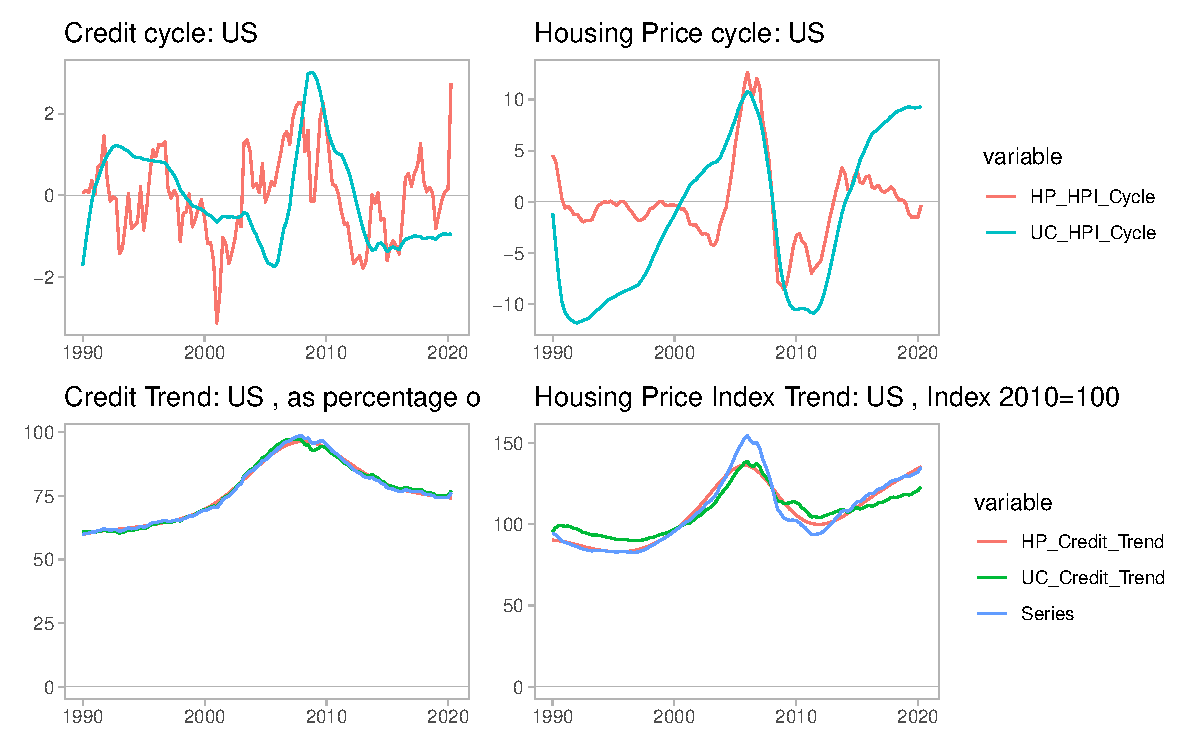
\includegraphics[scale=0.5]{../Regression/VAR_2/Output/Graphs/Combined_US}
		\end{minipage}
	\end{figure}
	
\end{frame}

%------------------------------------------------


\begin{frame}
	\frametitle{Key Results Regression Graphs: Great Britain}
	
	\begin{figure}[H]
		\begin{minipage}{0.95\textwidth} % choose width suitably
			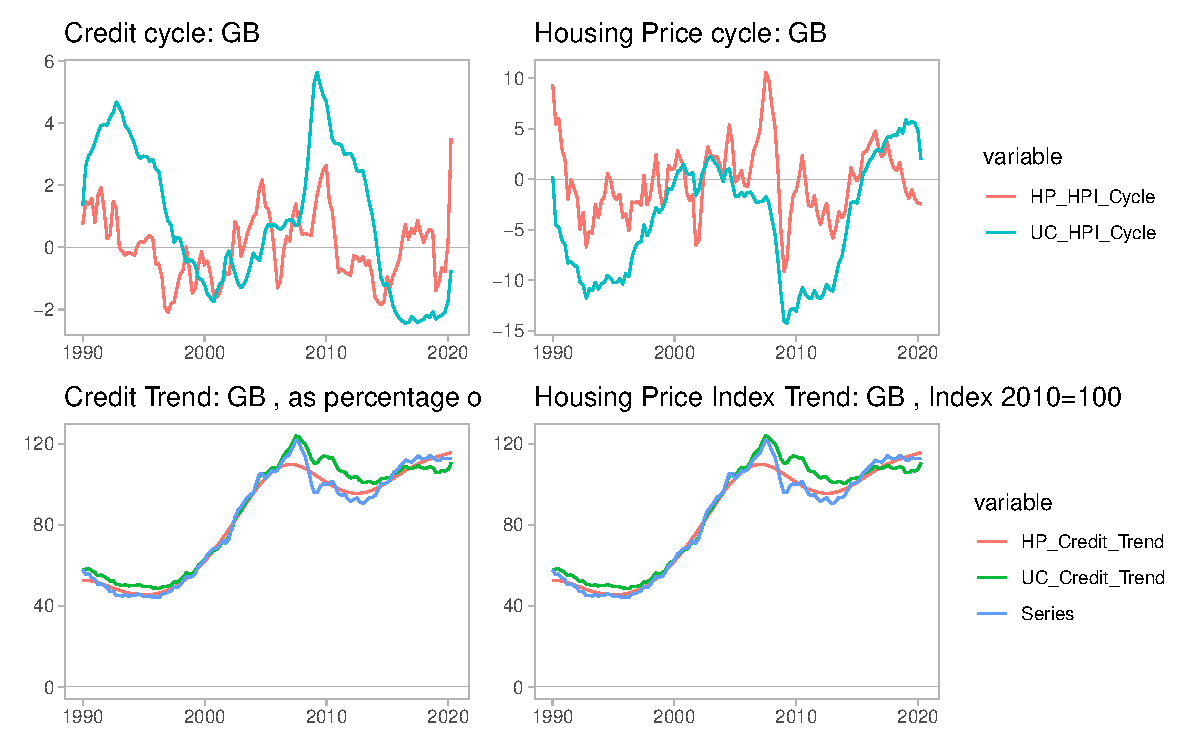
\includegraphics[scale=0.5]{../Regression/VAR_2/Output/Graphs/Combined_GB}
		\end{minipage}
	\end{figure}
	
\end{frame}


%------------------------------------------------


%\begin{frame}
%	\frametitle{Key Results RIF Decomposition: Evolution of Occupational Segregation - Manual Tasks}

%	\begin{figure}[H]
%				\begin{minipage}{0.95\textwidth} % choose width suitably
%					\centering
%		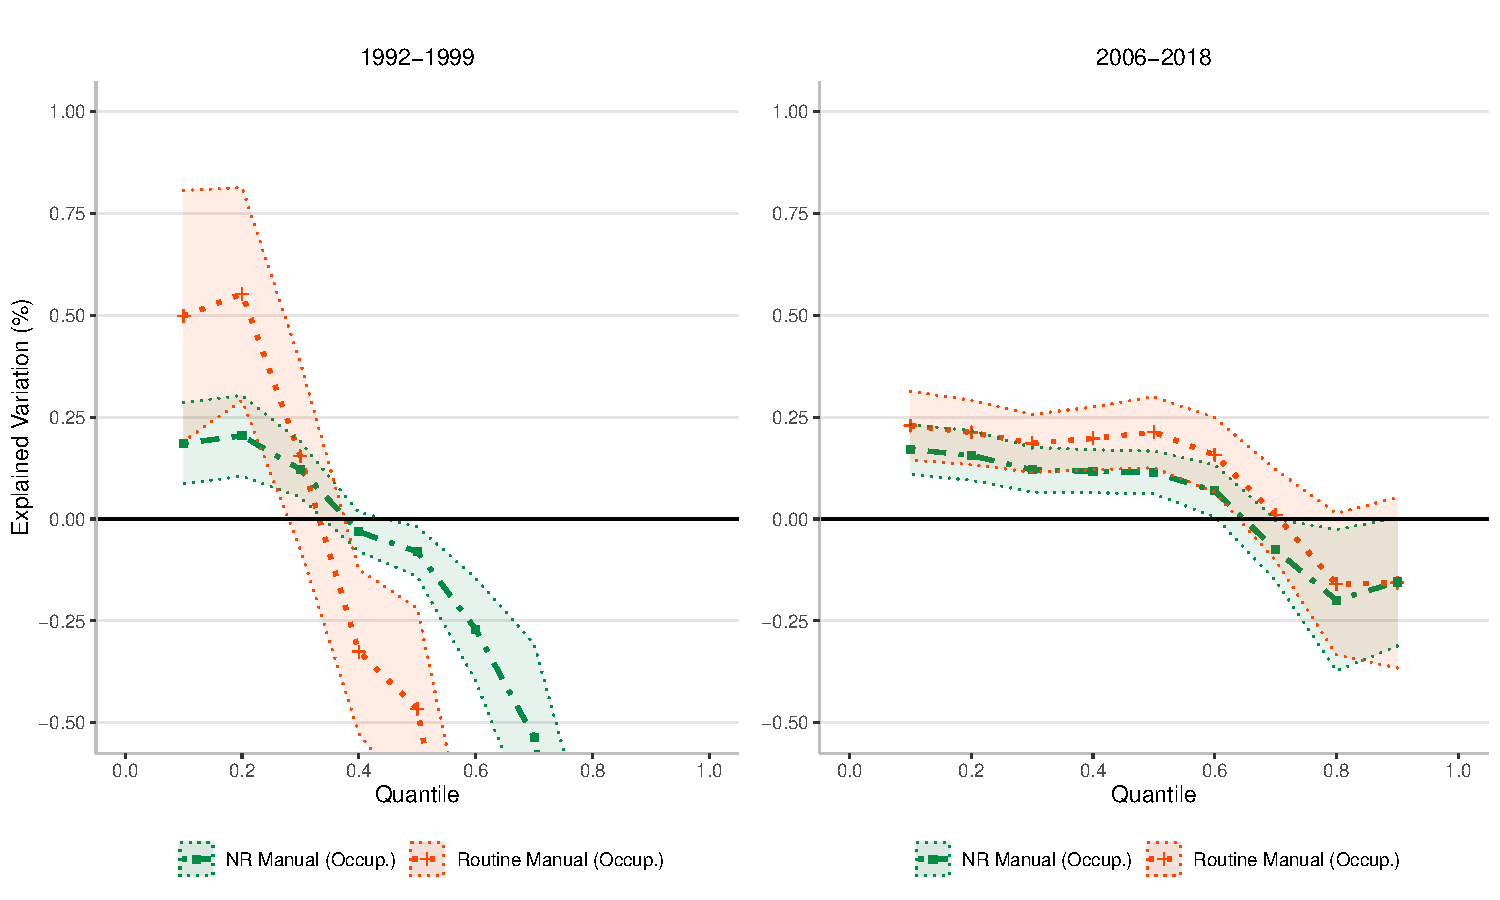
\includegraphics[scale=0.36]{rif_bw_man106}
%		\caption{Contributions of Individual-level variation in Tasks to the explained Wage Gap by Manual Tasks, 1992-2018 \label{fig:wgap_subs} \label{fig:wage_gap_base}}
%			{\footnotesize \tiny NOTE. \textemdash The decomposition results are top-censored for clarity, i.e. cut off at contributions of -50\% to the explained wage gap. \\ Point estimates are displayed with a 95\% Confidence Interval. \par}
%{\caption  {Contributions of Task Variation Within Occupations to the explained Native-Foreign Wage Gap with base task group Routine Manual, 1992-2018 \label{fig:wgap_within_baserm}}}
%				\end{minipage}
%	\end{figure}

%	\medskip

%	\begin{itemize} 
%		\item Decline in economic significance of occupational segregation
%	\end{itemize} 

%\end{frame}



%------------------------------------------------


%\begin{frame}
%	\frametitle{Key Results RIF Decomposition: Within-Occupation Task Specialization - Manual Tasks}

%	\begin{figure}[H]
%				\begin{minipage}{0.95\textwidth} % choose width suitably
%					\centering
%		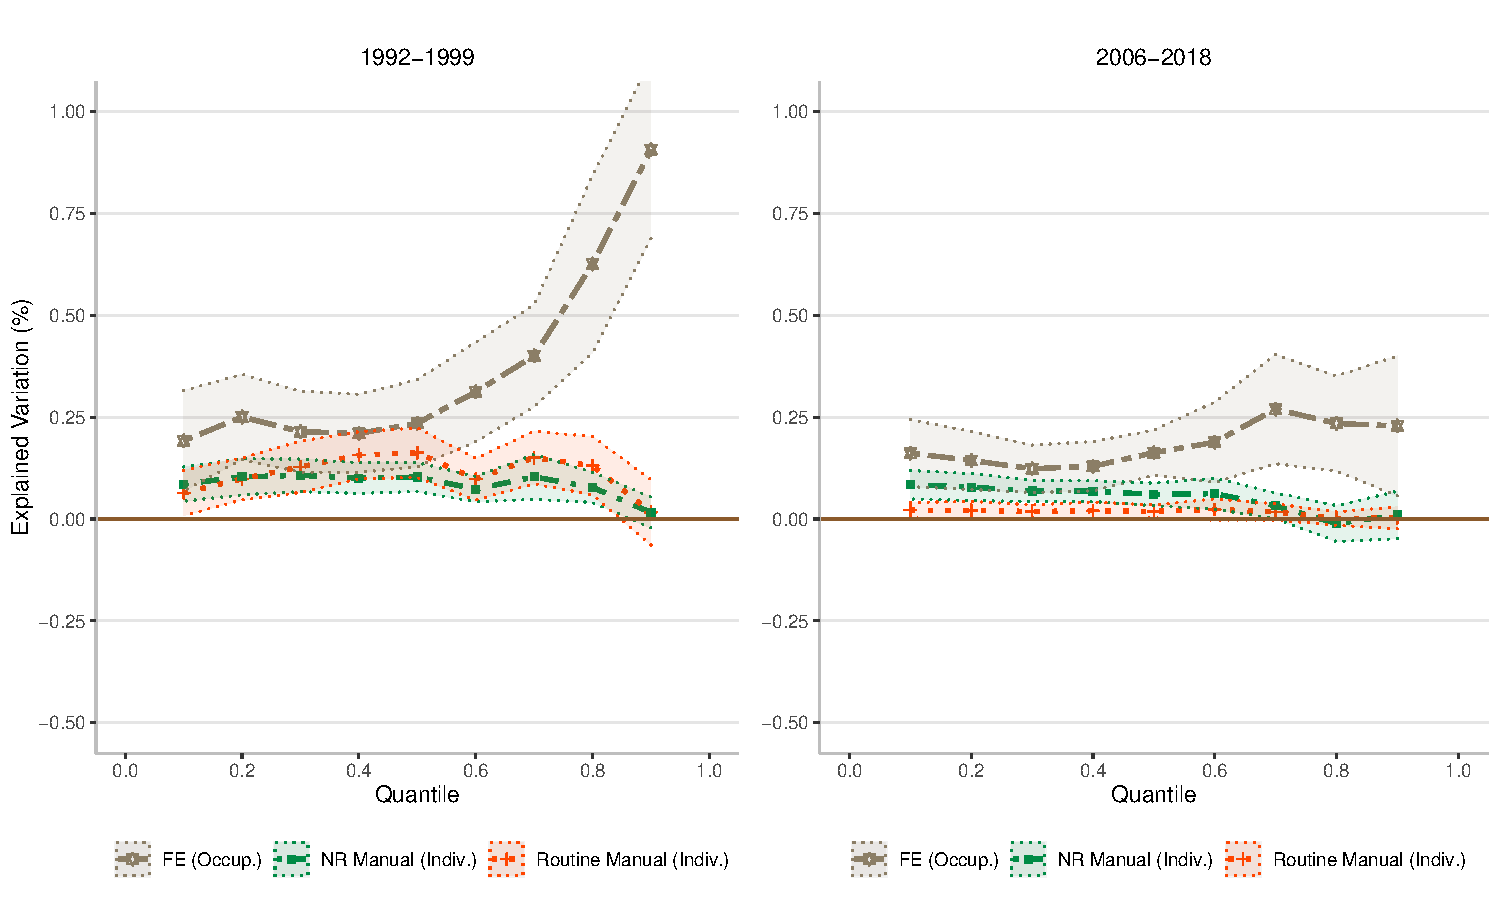
\includegraphics[scale=0.36]{rif_wi_man106}
%		\caption{Contributions of Individual-level variation in Tasks to the explained Wage Gap by Manual Tasks, 1992-2018 \label{fig:wgap_subs} \label{fig:wage_gap_base}}
%			{\footnotesize \tiny NOTE. \textemdash The decomposition results are top-censored for clarity, i.e. cut off at contributions of -50\% to the explained wage gap. \\ Point estimates are displayed with a 95\% Confidence Interval. \par}
%{\caption  {Contributions of Task Variation Within Occupations to the explained Native-Foreign Wage Gap with base task group Routine Manual, 1992-2018 \label{fig:wgap_within_baserm}}}
%				\end{minipage}
%	\end{figure}


%	\medskip

%	\begin{itemize} 
%		\item $IFEV_{NRI}^{0.8} (1992-99) = 0.2$ $\Longrightarrow$ $IFEV_{NRI}^{0.8} (2006-18) = 0.4$
%	\end{itemize} 

%\end{frame}


%------------------------------------------------


\begin{frame}
	\frametitle{Conclusions}
	
	\begin{enumerate}
		%\item \textbf{Native and Foreign Workers specialize in task assignments according to their comparative advantage}
		%	\begin{itemize}
		%	\item Natives specialize in abstract tasks involving problem-solving skills
		%	\item Foreigners specialize in manual tasks involving physical work
		%	\item Variation in interactive tasks has become an increasingly important determinant of the wage gap
		%	\item This trend is economically relevant within occupations, reinforcing already existing specialization patterns
		%	\item Future research should address differences in accumulation of human capital more formally \textbf{Bring Discusssion of Main Results in here}
		%	\end{itemize}
		%\medskip
		%
		\item \textbf{Dynamics of temporary components in housing and credit}
		\begin{itemize}
			\item Evidence showing that past movement of a cycle has predictive power over the other cycle
			\item Extracting temporary and permanent components information gave insights on the dynamics of the two series
		\end{itemize} 
		
		%Refined understanding for  small migration-induced wage effects: labor markets more segmented than previously assumed (key: incomplete transferability of human capital)
		
		\bigskip
		
%		\item \textbf{Implications on Immigration Policy}
%		\begin{itemize}
%			\item Federal Recognition Act (2012) \& Skilled Immigration Act (2020) aim at improving recognition of foreign qualifications
%			\item Findings suggest Policy Challenges with respect to 
%				\begin{itemize}
%					\item (i) Attraction \&
%					\item (ii) Retention of skilled immigrant workers
%				\end{itemize}
			%, but little success with programs involving occupation-specific skills
			%, especially of skilled foreign labor 
			
			%simplifies and standardizes procedures for the evaluation of foreign professional or vocational qualifications and opens up such procedures to target groups previously not entitled to pursue such a route, for example people from non-EU-countries. 
			
%		\end{itemize} 
		
		
	\end{enumerate}
	
	
	
\end{frame}


%------------------------------------------------


\end{document}